
\section{Experimental Tools}\label{method:tools}

In order to explore the large number of possible exchange instances described in
\S \ref{method:setup}, a sophisticated problem solving framework is needed. This
section describes the design principles and implementation details of a new
software package called Cyclopts (\underline{Cycl}us \underline{Opt}imization
\underline{S}tudies). Cyclopts, written primarily in Python with a C++ layer
used to operate with Cyclus, provides a general framework for sampling a
parameter space, defining problem instances for a given point in parameter
space, and solving a problem instance under a variety of conditions.

The section begins with a short discussion on terminology in \S
\ref{method:tools:term}.  \S \ref{method:tools:struc} describes the general
Cyclopts workflow and specific features used in the DRE experimental
campaign. \S \ref{method:tools:hdf5} discusses Cyclopts persistence mechanisms,
including database design and layout. The section concludes with \S \ref{},
describing Cyclopts' high throughput computing (HTC) capability, which enables
scalable, concurrent execution.

\subsection{Terminology}\label{method:tools:term}

Cyclopts supports a two-tier definition of problem instances, borrowing terms
from biological classification. Problem \textit{families} describe a general
form of problem instance. For example, the Traveling Salesman Problem (TSP)
could be implemented as a problem family. In this analysis, the NFCTP is
considered the problem family, since any given instance of the NFCTP will have
the same general structure. Whether or not the LP or MILP formulation is used is
dependent on whether or not arcs in the Exchange Graph are labeled as exclusive
or not. If there are no exclusive arcs, the LP formulation is used; otherwise,
the MILP formulation is used.

Each problem family can have any number of \textit{species}. One can
conceptualize the relationship as a tree structure, in which families are parent
nodes and species are child nodes. A problem species defines the methodology for
generating \textit{instances} of a problem family. Using the TSP example above,
a problem species may be ``the greater Atlanta metropolitan area'', for which
the effect of regional gas prices may be studied. For the NFCTP study, front-end
and back-end exchanges form two separate species. Each species can have unique
parameters in addition to family-related parameters, is the case for the two
species studied.

\subsection{Design}\label{method:tools:struc}

The full Cyclopts stack is comprised of three phases: generation of parameter
space, generation of instances, and execution of instances. The workflow begins
with user input detailing a range of values for a set of parameters. Cyclopts
then translates the input into a parameter space by enumerating all possible
combinations of parameters. For example, if parameters $x$ and $y$ have defined
values of $[1, 2]$ and $[3, 4, 5]$, respectively, Cyclopts will generate a
parameter space comprised of six points in $(x, y)$ notation: $(1, 3)$, $(1,
4)$, $(1, 5)$, $(2, 3)$, $(2, 4)$, and $(2, 5)$. Each point is then then
provided to a problem species in order to generate one or more problem
instances. Species are expected to define defaults for all parameters as user
input may define values for only a subset of available parameters.

Given a point in parameter space, an instance can be generated. If there are any
stochastic effects during instance generation, many instances may be
generated. Again, because parameters are species dependent, the logic of
instance generation from a set of parameters is the task of a problem
species. Following instance generation, instances may be executed. Cyclopts
supports multiple solution options by design. The same instance may be solved
with both a heuristic and a full optimization solver, for example. Once an
instance of a problem is defined, it is independent of any species-level
effects. Accordingly, instance execution and related logic is the domain of
problem families. 

A summary of the high-level Cyclopts workflow and entities is presented in
Figure \ref{fig:lopts_desgin}. Note that objects generated as the workflow moves
from parameter space to instance solution form a tree structure.

\TODO{update fig}
\begin{figure}
  \begin{center}
    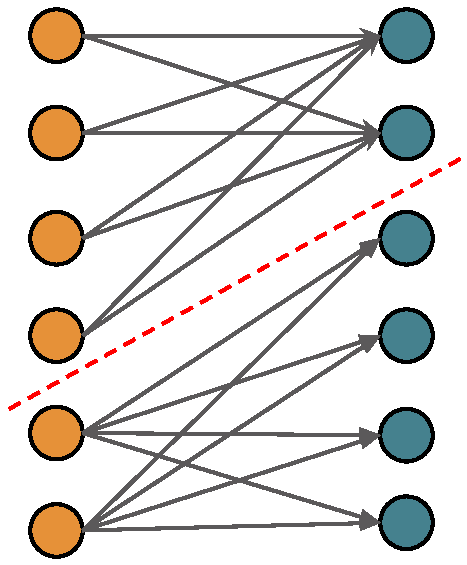
\includegraphics[width=0.55\textwidth]{exchange_part_supreq.pdf}
    \caption[]{
      \label{fig:lopts_desgin}
      Foo.}
  \end{center}
\end{figure}

\subsection{Persistence Mechanisms}\label{method:tools:hdf5}

While the root node in Figure \ref{fig:lopts_desgin} is generated from a
user-provided input file, each subsequent level in the hierarchy represents a
stateful object: a point in parameter space, a problem instance, and a
solution. Each stateful object can be written to and read from disc. Cyclopts
also incorporates a post-processing step, during which all related objects may
be analyzed and aggregate data may be collected and written to disc. While any
input/output (I/O) persistence mechanism is valid, Cyclopts is currently
implemented using HDF5 \cite{hdf5} via PyTables \cite{pytables}.

\subsubsection{Parameter Space}

\subsubsection{Problem Instance}

\subsubsection{Solution}

\subsubsection{Post Processing}

\subsubsection{Performance Studies}

\subsection{Implementation}

Cyclopts defines abstract application programming interfaces (APIs) for both
families and species in the \code{ProblemFamily} and \code{ProblemSpecies}
classes, respectively. While many parts of an API are related to the workflow
discussed in \S \ref{method:tools:struc:des}, others are related to the
persistence mechanisms discussed in \S \ref{method:tools:hdf5}.

\subsubsection{Problem Family}

Problem families are responsible for reading instances from a database, executing instances given a solver configuration, and writing solution 

\subsubsection{Problem Species}
 
\subsubsection{Exchange Family and Species}

\subsection{High Throughput Computing}\label{method:tools:htc}

Things \cite{bui_work_2011}.

\subsection{Command Line Interface}
